\documentclass[margin,line,a4paper]{resume}
 
\usepackage{polyglossia}
\setdefaultlanguage{danish}
\usepackage[none]{hyphenat}
\usepackage{graphicx,wrapfig}
\usepackage{url}
\usepackage{fontspec}
\usepackage{xltxtra}
\setmainfont{Minion Pro}
\usepackage[colorlinks=true, a4paper=true, pdfstartview=FitV,
linkcolor=blue, citecolor=blue, urlcolor=blue]{hyperref}
\frenchspacing
 
\begin{document}
\raggedright
{\sc \Large Curriculum Vitae -- Martin Bjeldbak Madsen}
\begin{resume}
    \vspace{0.5cm}
    \begin{wrapfigure}{R}{0.6\textwidth}
         \vspace{-1cm}
        \begin{center}
        \reflectbox{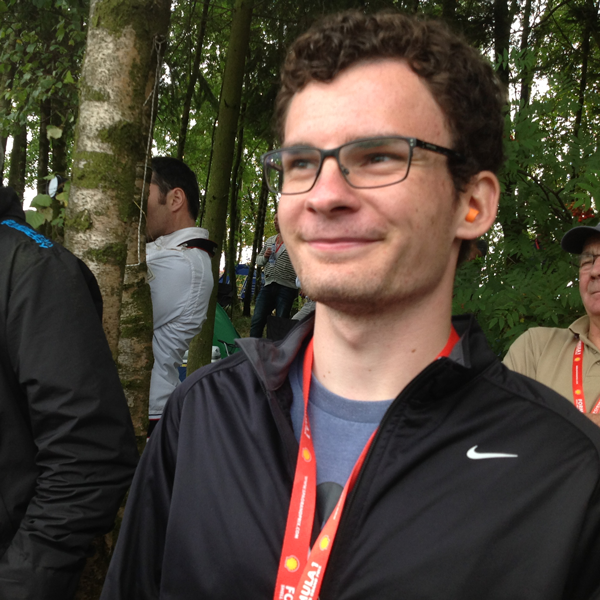
\includegraphics[width=0.6\textwidth]{moi.png}}
        \end{center}
         \vspace{-2cm}
    \end{wrapfigure}

    \section{\mysidestyle Personal\\Information}%\vspace{2mm}
    Martin B.\ Madsen\\
    June $9$th, $1992$ ($21$ years old)\\ 
    Langagervej 4, st 108\\
    9220 Aalborg Øst\\
    Denmark\\
    Mobile: +45 26 27 36 60\\
    \href{mailto:martin2madsen@gmail.com}{martin2madsen@gmail.com}\\
    \href{http://www.martinbmadsen.dk}{martinbmadsen.dk}\\
    \href{http://dk.linkedin.com/pub/martin-madsen/21/9b0/b0}{LinkedIn - Martin Madsen}
    \vspace{1cm}

    I was born and raised in Denmark until I was $5$ years of age,
    whereafter we moved for a total of $9$ years abroad, $4$ of which
    were spent in England, and $5$ in the US. That means that I'm quite
    used to speaking Danish and English with locals and can adapt to
    new cultural environments. Currently I live by myself and in the
    future, I see myself working in the tech, medicinal, or automotive
    industries.

    Currently I study Computer Science at Aalborg University here
    in Denmark. I attend $5$th semester and engage in interesting
    problem-based project group work along with following courses.
    As an example, we as a $6$-man group designed and implemented a
    programming language from the bottom up to make it easier for
    non-programmers to design board games. This semester is focused on
    machine intelligence, which piques my interest.

    \section{\mysidestyle Education}
    I have quite a normal educational background, except for the
    physical locations! Educational-wise, I plan to take the first year of
    my $2$-year master's in the US and then finish it at Aalborg University.

    \textbf{Aalborg University - Bachelor of Science, Computer Sience}
    ($2011$ - $2014$) I finish $6$th semester June $2014$ and will then
    have my bachelor's degree in Computer Science. My master's degree
    will be completed during the summer of $2016$.
      
    \textbf{EUC Nord - HTX} ($2008$ - $2011$) Technical gymnasium
    in Hjørring, Denmark. Finished the Higher Technical Examination
    Programme (HTX), a $3$-year vocationally oriented general upper
    secondary programme, and a prerequisite for admission to higher
    education. I took the highest level Math, Physics, English, and
    Danish possible.
    
    \textbf{Bagterpskolen} ($2006$ - $2008$) Completed the Danish
    Folkeskole Education in Hjørring, Denmark.

    \textbf{J. R. Gerrits Middle School} ($2003$ - $2006$) Elementary and 
    Middle School i Kimberly, Wisconsin, USA.

\pagebreak
\section{\mysidestyle Professional\\experience}\vspace{1mm}
\begin{description}

  \item[September 2012 $\rightarrow$ now] Student programmer at Falck
  Healthcare a/s. I took over the development of a web app used by
  Falck's physiotherapists when journaling their contact with patients.
  I spend around $15$ hours per week working there alongside my studies.

  \item[Sept 2010 $\rightarrow$ now] Run my own company,
    \emph{Divambu}. Here I develop and host web sites for small companies.
    By visiting \url{divambu.dk}, you can see a portfolio of some of the
    projects I've worked on.

  \item[October 2008 $\rightarrow$ June 2010] Service worker at
    Fakta a/s (part of Coop Denmark). Was in direct contact with customers
    and fulfilled everyday tasks required to run a busy grocery store. I
    worked during evenings, weekends, and holidays alongside attending
    school full-time while I was under 18.
\end{description}

\section{\mysidestyle Other activity}\vspace{1mm}
\begin{description}
  \item[July 2012 $\rightarrow$ now] Mentor, Project
    \href{http://www.urk.dk/solskinsunge/}{Solskinsunge} $2012$. Volenteer
    work, where we arrange bi-monthly social gatherings for teenagers aged
    $15 - 18$, most of which are second generation immigrants.
\end{description}
Furthermore, I was responsible for contacting organizations and
companies to gather sponsorships for a software development camp hosted
by UNF, The Danish Youth Association of Science in the summer of $2013$.
During the week-long camp itself, I helped the mostly young participants
with any problems they might have had when developing their Android
applications.

In January $2013$, I was elected to sit on the Study
Board for Computer Science at Aalborg University
(\href{http://www.en.sict.aau.dk/Study+board+for+Computer+Science/}{link}).
Here we take on responsibilities for bachelor and master programs
within the following educations Computer Science, Informatics,
Information Technology, Software Engineering, and Software Construction
and their curricular. Here we receive and discuss, among others,
qualification and exemption applications, quality assurance of the above
educations.

I've had a Danish driver's license for $3$ years.

\section{\mysidestyle Skills} \vspace{1mm}
I can quickly involve myself in new material, but there are a few
technologies and systems I have more experience with than others:
\vspace{0.5cm}
\begin{description}
  \item[Operating systems] Basic understanding of most Unix-like
    systems: Ubuntu, Debian, CentOS, Arch Linux, Mac OS X.
  \item[Servers and databases] Nginx. 
  \item[CMS-systems] I've set up systems with Wordpress, phpBB,
    Octopress.
  \item[Revision control] Git, SVN.
  \item[Programming, scripting, and markup languages] \LaTeX\ and
    \XeTeX, HTML, CSS, C, C$\sharp$, Java, JavaScript and jQuery, Ruby
    and Ruby on Rails.
\end{description}

\pagebreak
\section{\mysidestyle Language}
My native language is Danish, but almost everything I write and read is
in English, both academically at university and merely communicating to
others when I'm at home, coding or not.

\begin{description}
  \item[Danish] first language
  \item[Spoken English] fluent
  \item[Written English] fluent 
\end{description}

\section{\mysidestyle Interests}
When I'm not in front of my computer, I love to enjoy a cup of tea and read non-fiction. There is also nothing better than travelling the world, so I try to do that as much as possible, and thankfully due to my fantastic friends, I've had quite a few fantastic experiences travelling to visit then. I also enjoy electronic and classical music, such as house and Tchaikovsky. Keeping my body healthy and in shape is also important to me, so naturally I quite enjoy cooking sexy, irresistable food!
\end{resume}
\end{document}
